\section{Fixed-Point RTL Reference Model}
\label{sec:fixed}

\texttt{ofdm\_phy/fixed/} is an integer-only twin of the modem,
structured the way an FPGA/ASIC datapath would be.  It is the golden
reference a future RTL implementation verifies against;
\texttt{experiments/fixed\_point.py} (24 checks,
Appendix~\ref{app:fixed}) cross-validates it against the float model
continuously.

\subsection{Receiver Datapath}

Figure~\ref{fig:fixed_rx} shows the complete integer receive path,
from int16 audio to decoded packet.  The model covers the \emph{full}
frame family: convolutional and LDPC FEC, BPSK/QPSK/16-QAM, all three
link modes, HARQ chase combining, and the optional calibrated-LLR
mode --- on the transmit side as well:
\texttt{build\_frame(fec="ldpc")} emits \texttt{ver=2} frames (the
LDPC accumulator encoding is already pure integer, so only the
header/codec switch was needed), and the Q15 constellations cover
BPSK, QPSK, and Gray 16-QAM (per-axis levels
$\{\pm 1, \pm 3\}/\sqrt{10}$).

\begin{figure}[H]
    \centering
    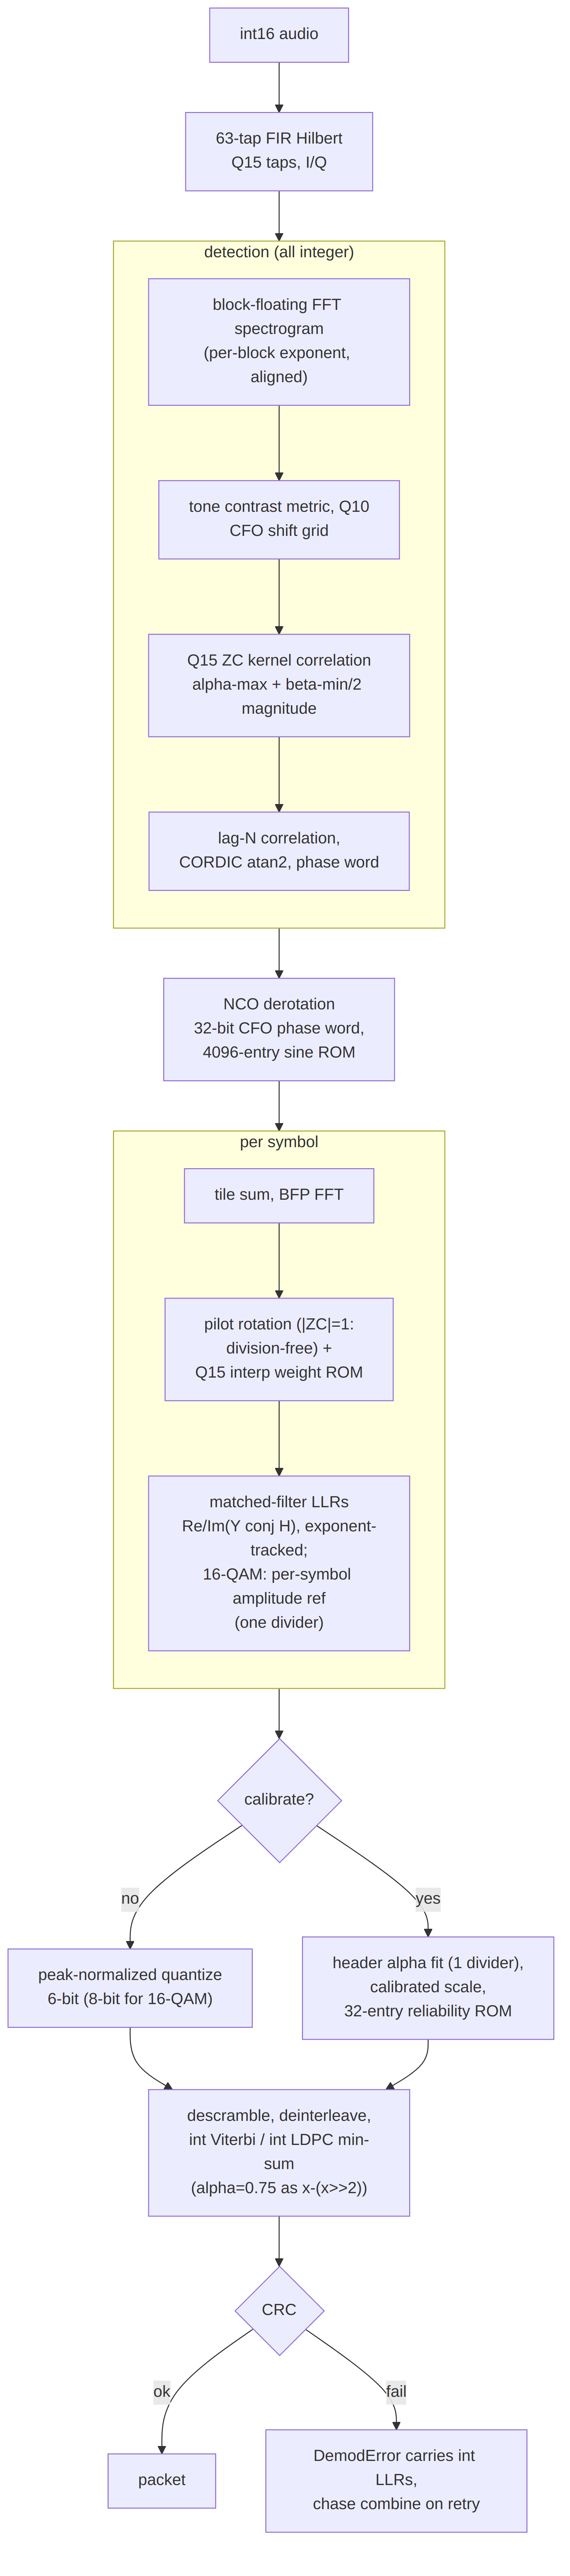
\includegraphics[width=0.8\textwidth,height=0.62\textheight,keepaspectratio]{images/fixed_rx.png}
    \caption{Fixed-point receiver datapath (all integer).}
    \label{fig:fixed_rx}
\end{figure}

\subsection{Primitive Blocks}

\begin{table}[H]
    \centering
    \caption{Fixed-point primitives and their measured quality.}
    \label{tab:fixed_prims}
    \small
    \begin{tabular}{@{}lp{7.2cm}l@{}}
    \toprule
    \textbf{Block} & \textbf{Structure} & \textbf{Quality} \\
    \midrule
    FFT     & radix-2 DIT, Q15 twiddle ROM, per-stage $\gg 1$
              (built-in $1/N$), BFP wrapper & 59\,dB SQNR \\
    Hilbert & 63-tap type-III FIR, Q15 & 61\,dB SQNR \\
    NCO     & 32-bit phase accumulator, 4096-entry Q15 sine ROM &
              $-67$\,dBc \\
    CORDIC  & 16-iteration vectoring, angle in phase-word units &
              $<0.001$\,rad \\
    Viterbi & 6-bit LLRs (8-bit for 16-QAM data), $\pm 1$ expected
              symbols (adds only), int32 metrics & exact \\
    LDPC    & integer normalized min-sum,
              $\alpha = x - (x \!\gg\! 2)$ & matches float min-sum \\
    \bottomrule
    \end{tabular}
\end{table}

\subsection{RTL-Oriented Conventions}

\begin{itemize}
    \item \textbf{CFO is a 32-bit phase-increment word} end-to-end (one
          turn $= 2^{32}$); Hz exists only at API boundaries.
    \item \textbf{Divisions are minimised.}  Channel estimation is
          division-free ($|$ZC pilot$| = 1$, so the estimate is a
          rotation); pilot interpolation is a Q15 weight ROM.  The
          remaining dividers: the calibration $\alpha$ fit (one per
          frame), the 16-QAM amplitude reference (one per symbol), and
          the detection metrics.
    \item \textbf{Scale tracking.}  BFP exponents are carried through
          every energy and LLR comparison (scale
          $\propto 2^{2\cdot\mathrm{exp}}$); ZC correlation magnitude
          uses the $\alpha$-max~+~$\beta$-min/2 approximation.
\end{itemize}

Two intentional deltas versus the float model: NORMAL-mode tone
detection uses a 256-point FFT (float: 128) so the coarse CFO grid is
fine enough for an unambiguous lag-$N$ residual; and the demodulator
uses the slew-limited frequency-search tracker for \emph{all} tile
factors --- the float model's polynomial phase fit is not RTL-friendly,
and measurably weaker at the edge anyway.

\subsection{Measured Results and One Surprise}

The fixed TX waveform correlates 0.99998 with the float waveform; the
full fixed/float TX$\times$RX cross-matrix decodes; NORMAL-mode PER is
within $\approx$0.5\,dB of the float receiver, and ROBUST/EXTREME
decode at $-11/-17$\,dB.  The surprise: the default 6-bit
peak-normalized LLR quantization already acts as a \emph{compressive
recalibration} (Section~\ref{sec:llr}), and combined with the
frequency-search tracker the fixed receiver \textbf{matches or beats
the recalibrated float chain at $-9/-10$\,dB} (22 vs.\ 20 and 11 vs.\ 5
of 30 trials).  The calibrated-LLR mode (integer header $\alpha$ fit
plus a 32-entry reliability ROM measured on the fixed chain itself)
therefore buys a \emph{stable cross-frame LLR scale} --- what makes
HARQ combining legitimate --- rather than extra PER.

The 16-QAM rungs were swept separately
(\texttt{experiments/fixed\_qam16\_sweep.py}, 48 packets/point, fixed
TX with identical samples into both receivers).  The first sweep
exposed a $\sim$2\,dB gap on the puncture-weak high rates
($+4.6/+6.3$\,dB versus float $+2.6/+4.5$ at rates 2/3 and 3/4):
16-QAM max-log LLRs span a much wider dynamic range than BPSK
(inner/outer bits times per-carrier gain), and the 6-bit
peak-normalized quantization compresses them.  The fix is a
\emph{per-modulation quantizer}: data blocks with $\mu = 4$ use an
8-bit peak-normalized quantizer ($\pm 127$), while $\mu \le 2$ keeps
the 6-bit path, whose compression is precisely what helps at the BPSK
edge.  Peak and mean normalization measured equivalent at 8 bits ---
the win is the resolution --- so the RTL cost is two extra LLR bits on
the 16-QAM data path only.  Re-swept, the fixed receiver measures
$+1.5/+2.9/+5.3$\,dB for rates 1/2, 2/3, 3/4: within 0.3--0.8\,dB of
the float receiver everywhere.

Robustness note: the tiled chain survives up to 65\,\% contiguous
audio erasure (the $4\times$ tiles keep partial symbols alive); the
HARQ path is validated by a deterministic test with two 75\,\%
complementary erasures whose union covers every sample at least once.

\subsection{Gated Two-Stage Frequency Search}

The first-symbol residual-CFO search --- 275 full-symbol hypotheses at
EXTREME, the demodulator's dominant burst in a firmware budget --- was
restructured as coarse-then-fine: a quarter-length coarse pass
(tiles/4 accumulation, whose $4\times$ wider frequency mainlobe
tolerates a $4\times$ coarser grid) ranks hypotheses, and only the
top-3 $\pm 5$-step windows run at full precision, $\approx$5.5$\times$
fewer derotated samples.  The coarse metric is $\sim$6\,dB noisier
than the full symbol, and a hard coarse decision measurably costs
$\sim$0.5\,dB at the EXTREME sensitivity edge --- so the fast path is
taken only when the coarse top-1/median contrast clears a measured
gate ($2.25\times$; edge frames sit $\le 2.2\times$, frames with
5\,dB of margin $\ge 2.7\times$), and below it the exhaustive grid
runs unchanged.  The same gated structure was then back-ported to the
\emph{float} demodulator's per-symbol frequency search --- where it
pays on every symbol, not just the first, because the float chain has
no slew-limited tracker.  Figure~\ref{fig:coarse_ab} shows the
noise-sensitivity A/B (\texttt{experiments/coarse\_search\_ab.py},
36 packets/point, identical channel realizations per arm), including
the ablation that justifies the gate: the quarter-length coarse pass
\emph{without} the gate (dotted) shifts the EXTREME waterfall right by
0.5--1\,dB (fixed RX at $-18$\,dB: PER 0.31 vs.\ 0.11), while the
gated search (dashed) is \emph{identical} to the exhaustive grid at
every measured point, both models --- lossless by construction, with
the full grid reduced to a low-margin fallback.  ROBUST tolerates
even the ungated coarse pass at parity: its coarse stage (4 of 16
tiles) retains enough detector SNR at that mode's shallower edge, so
the gate specifically protects the deepest mode.

\begin{figure}[H]
    \centering
    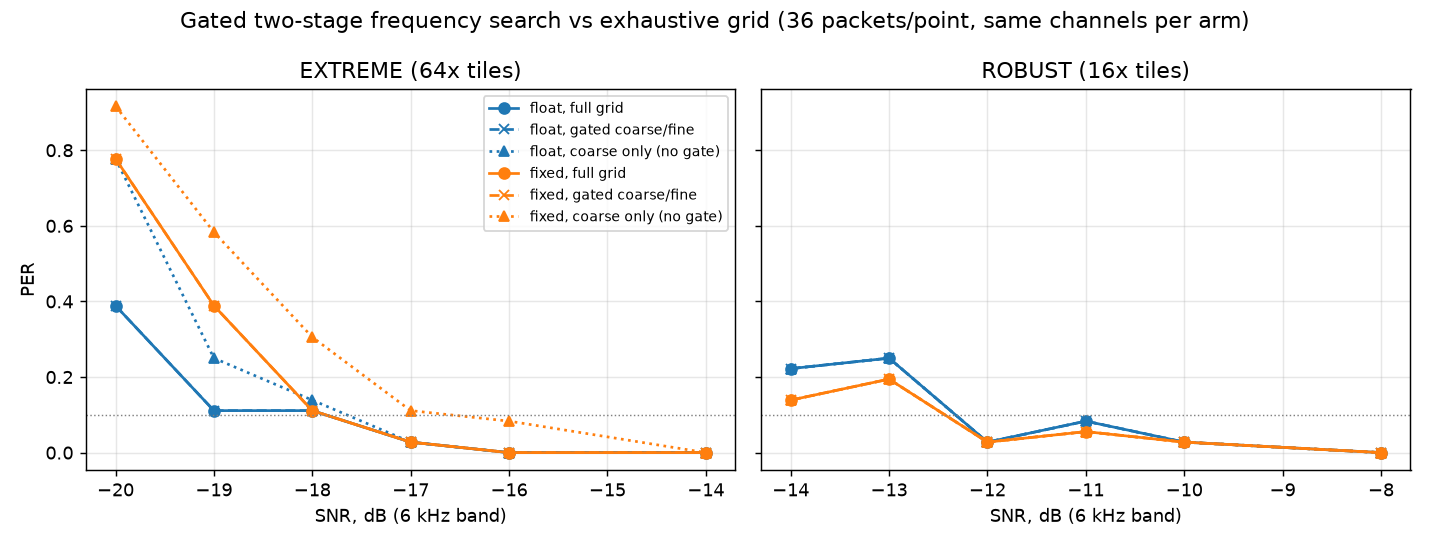
\includegraphics[width=\textwidth]{images/coarse_search_ab.png}
    \caption{PER versus SNR for the exhaustive frequency grid (solid),
             the gated two-stage search (dashed), and the ungated
             coarse-only ablation (dotted); float and fixed-point
             receivers, same channels per arm.  Gated overlays full
             exactly everywhere; the ablation's edge loss in the
             EXTREME panel is what the contrast gate prevents.}
    \label{fig:coarse_ab}
\end{figure}

\subsection{Integer SNR Estimator and Full-System Integration}

Rate adaptation is driven by a per-frame SNR estimate the fixed
receiver originally lacked.  The added estimator is data-aided and
divider-free: per-column first/second moments of the LLR stream
against the known $\pm 1$ bits (the re-encoded header always, plus the
decoded data block for $\mu \le 2$), an integer $\log_2$ via bit-length
and a 16-entry mantissa ROM, minus the tiling gain, plus one measured
global calibration constant ($-7.2$\,dB, constant across all modes and
modulations).  Two design points were forced by measurement.  First,
grouping moments \emph{per column} removes the multipath $|H|^2$
spread across carriers.  Second, symbol rows must be
\emph{gain-weighted} by their mean $|$LLR$|$: a tiled EXTREME frame
spans several QSB fade cycles, and both naive poolings failed ---
unweighted moments count the fading itself as noise (measured
5--15\,dB pessimistic, which parked the rate ladder at rung~0), and
equal-weight gain-normalized pooling yields a harmonic-mean-flavored
estimate still dominated by fade valleys.  Gain weighting reproduces
the signal-energy-weighted average the float estimator reports --- the
statistic the ladder was tuned against --- and reduces to the plain
estimator when the gain is constant.  Final accuracy:
$\le$1.5\,dB error over $-17\ldots+8$\,dB, every mode and modulation
(slightly pessimistic on the tiled modes, the safe direction).

With the estimator in place, a thin adapter (\texttt{FixedPHY}) gives
the fixed TX/RX the float \texttt{Transceiver}'s link-facing interface
--- including blind mode auto-detection by trying the three per-mode
receivers --- and \texttt{LinkStation} accepts it via a \texttt{phy}
parameter.  The complete adaptive system then runs on the integer
pipeline end to end: \texttt{demo\_wav.py -{}-phy fixed} records the
two-station QSO of Section~\ref{sec:results} with both stations
\emph{and} the blind monitor decoding on fixed point.  At
$-2/-1$\,dB the session bootstraps at EXTREME, netting and climbing
exactly as the float system does, and the monitor blind-decodes 37 of
47 frames; at $+5$\,dB the ladder climbs into 16-QAM (rungs 9--10 on
the air, requests up to rung~11) and the monitor decodes 26 of 40
(Appendix~\ref{app:fixeddemo}).

\subsection{Debug Lore}

Three integer-domain bugs cost real time and are recorded so an RTL
implementation does not repeat them: the ZC metric's Q-scaling must
account for \emph{both} $2^{-15}$ factors the Q15 kernel introduces (a
perfect correlation scored 0.006 with one missing); scipy's
\texttt{remez(..., type="hilbert")} returns taps producing $-\sin$ for
a cosine input, so the taps must be negated for a positive-frequency
analytic signal; and BFP energies compare only after shifting by
$2\,\Delta\mathrm{exp}$.
